\chapter{Background}
    In this chapter, the key concepts used during the experiments will be introduced. Afterwards, the context of the research field will be described.  
    
\section{Terminology Of Multidimensional Arrays}
    This chapter will frequently describe multidimensional arrays; therefore this section will clarify some commonly used terms. Multidimensional arrays consist of multiple 2-dimensional arrays. These are called \textit{channels}, and have uniform \textit{resolution}. \textit{Depth} denotes the number of channels, while the resolution indicates the \textit{height} and \textit{width} of the channels. Thus, a multidimensional array can be described with \textit{height} x \textit{width} x \textit{depth}. The terms are illustrated in figure \ref{Multidimensional array terminology}.
    
        \begin{figure}[H]
        \centering
                        \includesvg[inkscapelatex=false,width=0.8\textwidth,keepaspectratio]{figures/n_array_terminology.svg}
        \caption[Multidimensional  array]{Illustrations of the resolution (\textit{height} and \textit{width}), and \textit{depth} of a multidimensional array where the depth is split into \textit{channels} (different colors). In this example, the resolution is 3×3 and the depth is 4. }
      	\medskip 
        \label{Multidimensional array terminology}
    \end{figure}
    

\section{Echosounder and Image Data} \label{echosounder and image data acoustic }
    This section describes the data gathered by the Simrad EK60 echosounder system produced during the yearly trawl surveys conducted by the \gls{imr}\cite{johnsen2017collective} and how it relates to image data. Echosounders are maritime instruments, in this case mounted below a ship, which emit acoustic waves into the water (\textit{ping}) and log the backscattered waves\cite{brautaset2020acoustic}. The logs record the \gls{sv}. The data is 2-dimensional, recording the \textit{date and time of the ping} and \textit{range} (\textit{depth}) of the backscattered waves, for each frequency channel used during the measurement. This output is called an \textit{echogram}. As the ping rate was set to 1Hz\cite{choi2021semi}, with a pulse duration of 1.024 milliseconds, the length of each pixel is 1 second horizontally and 19.2 centimeters vertically. These echograms represent some visible observation of the water column below the echosounder, and because of this, each frequency channel can be viewed as similar to color channels in a picture. Hence, machine learning techniques usually applied to image data are also applicable to \textit{echograms}. Figure \ref{accoustic data and color channels fig} illustrates an example of this:

    \begin{figure}[H]
        \centering
        
        \subfloat[Frequency channels that form an echogram. This example show an example \gls{sv} data crop with six frequencies, on the log scale.]{
        	\includesvg[inkscapelatex=false,width=0.4\textwidth,keepaspectratio]{figures/freq_stacked.svg}}
        	%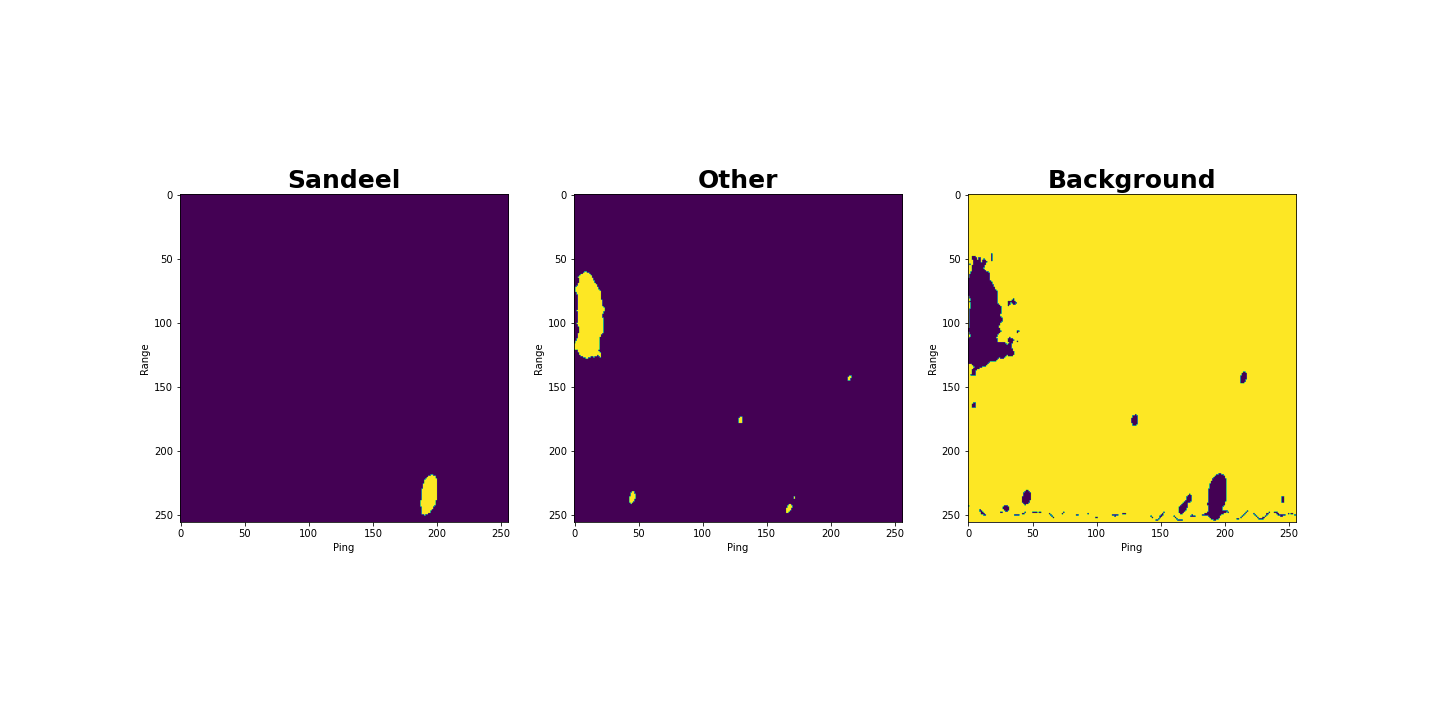
\includegraphics[width=1\textwidth]{figures/data_sample.png} } 
        
        \subfloat[Color channels RGB that forms a picture.]{
        	\includesvg[inkscapelatex=false,width=0.9\textwidth,keepaspectratio]{figures/colors_and_OG.svg}}
        
        
        \caption[Frequency channels and color channels]{(a) and (b) both consist of several channels that together represent some visual observation.}
        \label{accoustic data and color channels fig}
        
        \end{figure}
    
    More information about the acoustic data used in this thesis is contained in section \ref{unet_paper_acoustic}.
    
\clearpage
\section{Machine Learning} \label{Machine Learning}
    As described in the book Deep Learning\cite{Goodfellow-et-al-2016_ML}, machine learning can intuitively be split into four parts; the \textit{algorithm}, \textit{empirical data}, a \textit{task} and a \textit{performance} measure. A machine learning algorithm is designed to increase its performance on a task, given data. During this process also called \textit{training}, the algorithm is said to be \textit{learning}. Afterwards, it outputs a \textit{model} which represents what the algorithm learned and can predict on new data. Machine learning approaches can be divided into three categories\cite{Goodfellow-et-al-2016_E}: supervised learning, unsupervised and reinforcement learning. 
    
    \subsection{Algorithm approaches} \label{Algorithm types}
        \subsection{Supervised learning}
            Supervised learning \cite{Goodfellow-et-al-2016_E} algorithms are defined by the fact that the training data consists of the input and a desired output. This means that the algorithm will have to learn a function, mapping from input to correct output. In classification problems the output would be a class label, while in regression problems the output is a value within a numerical range (for example, predicting the height of a person).
            
        \subsection{Unsupervised Learning}
            Unlike supervised leaning, unsupervised learning algorithms only receive the input and learn properties contained in the data\cite{Goodfellow-et-al-2016_E}. A practical example is clustering, where the dataset is divided into clusters based on similar features. 
                
        \subsection{Reinforcement Learning}
            In reinforcement learning \cite{Goodfellow-et-al-2016_E}, the algorithm does not learn from a given dataset, but actsin an environment. In some cases, this is a feedback loop, giving either a positive or negative reward for performing certain actions. The goal is then for the algorithm to maximize this reward. This is what people often associate with \gls{ai} and can for example be seen in the AlphaZero software that beat professional chess players\cite{silver2017mastering}.
    
    \subsection{Data and Features}
    \citeauthor{najafabadi2015deep}\cite{najafabadi2015deep} state that the quality of the input data to a machine learning algorithm will likely affect its performance. Hence, time allocated to increase quality of the data can exceed the time spent learning.  Data must be gathered, integrated, cleaned of errors, preprocessed, and features extracted before being input to the algorithm. The process of extracting features is often referred to as \textit{feature engineering}. It constructs a representation of the data with the best factors to solve the task. This is often domain specialized, and usually involves human involvement. In section \ref{neural networks}, \gls{ann} are introduced, which have the ability to automate extraction of complicated features.

    \subsection{Model Evaluation}
    As mentioned, a machine learning algorithm needs a performance measure and will be described in this section. First, a technique applied to measure different aspects of the model. Followed by some usual behavior we can observe in these measurements. Finally, the \textit{performance metric} itself will be described and how it is estimated. 
    
    \subsubsection{Train-Validation-Test Split}
        The goal, when a machine learning model is learning, is to achieve the lowest \textit{generalization error}\cite{Goodfellow-et-al-2016_generalization} (formula and metric provided later in this section). This means to not only perform well on data seen during training, but also on new unseen data. To measure this, it is normal to split our data into three parts\cite{Goodfellow-et-al-2016_train_val_test_split}: the \textit{training}, \textit{validation} and \textit{test} dataset. As the name suggests, the training data is used during the training process of the model, in which the model seeks to minimize the training error. The validation dataset, is extracted from the training dataset and can for example be used to evaluate different models against each other. Finally, the test dataset is used to get an unbiased estimate of the final selected model's \textit{generalization error}.
        
    
    \subsubsection{Overfitting Vs. Underfitting}
        As stated by \citeauthor{Goodfellow-et-al-2016}\cite{Goodfellow-et-al-2016} the performance of a model is dependent on its \textit{training error}, and the difference between this \textit{training error} and the \textit{test error}. \textit{Underfitting} happens when a model fails to achieve a low training error, while \textit{overfitting} happens when the difference between the test error is segnificantly lower than the training error. To manipulate this behavior, we introduce \textit{capacity}. Capacity is the likelihood of the model either underfitting or overfitting, and it controls the complexity of the model.  Low \textit{capacity} means that the model fails to capture patterns contained in the data. High \textit{capacity} translates to adjusting to the training data to such an extent that the model performs worse when given unseen test data. The optimal solution, depicted in the center plot of figure \ref{over/under fit fig}, is to have a model with a balanced capacity that is as close to the true function as possible. 
        
        \begin{figure}[H]
            \centering
            %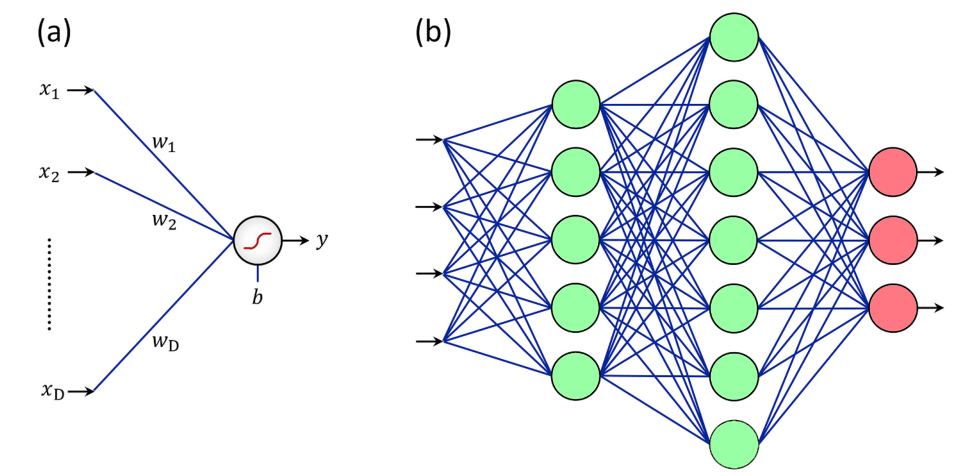
\includegraphics[scale=0.5]{figures/perceptron.png}
            \includesvg[inkscapelatex=false,width=1\textwidth,keepaspectratio]{figures/overunderfit.svg}
            \caption[Over/under-fit]{Training data is generated with random noise around a sinus wave (True function). Model \textit{capacity} increases from left to right. The center plot illustrates a model that have learned an almost perfect fit to the actual true function.}
          	\medskip 
            \label{over/under fit fig}
        \end{figure}
        
    \subsubsection{Performance Metrics} \label{f1_score}
        This section describes the performance metrics used in this thesis. Consider a binary classification system that classifies samples into either the \textit{positive} or \textit{negative} class\cite{powers2020evaluation_f1_recall_precision}. Predictions by the classifier can thus be sorted into the following four categories:
        
        \begin{itemize}
            \item \textbf{True positive (TP):} A correct classification of a positive example.
            \item \textbf{True negative (TN):} A correct classification of a negative example.
            \item \textbf{False positive (FP):} A negative example incorrectly classified as positive
            \item \textbf{False negative (FN):} A positive example incorrectly classified as negative.
            \end{itemize}
        
        We can now calculate the performance of the classifier from these values, and the simplest is accuracy\cite{powers2020evaluation_f1_recall_precision}:
        
        \begin{equation}
            accuracy = \dfrac{\textrm{\textit{correct predictions}}}{\textrm{\textit{total number of predictions}}} = \dfrac{TP+TN}{TP+TN+FP+FN} 
        \end{equation}
        
        This metrics does not handle class imbalance well\cite{powers2020evaluation_f1_recall_precision}, as it is equivalent to calculating the percentage of correct predictions. The example being that if 95\% of the data belongs to one class, then always predicting this class will give us an accuracy of 95\%.
        
        To deal with class imbalance, we calculate two new metrics, \textit{precision} and \textit{recall}\cite{powers2020evaluation_f1_recall_precision}. Precision is the percentage of positive predictions made by the model that are correct. Recall is the percentage of all positive samples the model managed to classify correctly.
        
        \begin{equation}
            \textrm{\textit{precision}} = \dfrac{TP}{TP+FP}
        \end{equation}
        
        \begin{equation}
            \textrm{\textit{recall}} = \dfrac{TP}{TP+FN}
        \end{equation}
        
        Then, by using precision and recall, we calculate the \textit{F1-score}\cite{powers2020evaluation_f1_recall_precision}. It combines these metrics and is designed to work well on imbalanced data. There are of course many other performance metrics, but this section will be limited to describing those used in the thesis. The F1-score formula:
        
        \begin{equation}
            \textrm{\textit{F1-score}} = 2 \cdot \dfrac{\textrm{\textit{precision}} \cdot \textrm{\textit{recall}}}{\textrm{\textit{precision}} + \textrm{\textit{recall}}}
        \end{equation}
        

\section{Artificial Neural Networks} \label{neural networks}
    In this section, we introduce the basic components of an \gls{ann} and how these are combined to create a \textit{deep learning} network. 

    \subsection{Perceptron} \label{perceptron}
        The \gls{ann}s fundamental building block is called an artificial \textit{neuron} or perceptron. It is formulated in the following way\cite{razavi2021deep_exp_per}:
            \begin{equation} \label{eq_perceptron}
                y = \sigma(\sum_{i=1}^{D}w_ix_i + b)
            \end{equation}
            
        where D is the number dimension of the input space, $x$ is the input vector and $w$ is a set of weights that is of the same size as $x$, $b$ is the bias and {\textsigma} is a nonlinear activation function which will be explained later in \ref{activation function}. The output \textit{y} is a weighted sum of the input and weights, also called the neurons' \textit{activation}. In short, the equation inside the activation functions is a linear regression with the tunable parameters $w$ and $b$. The perceptron is illustrated in figure \ref{Perceptron / MLP}.
    
    \subsection{Multi-Layered Perceptron} \label{MLP}
        The neurons presented in section \ref{perceptron} are organized together in layers to form a \gls{ann}, which in turn forms what is called a \gls{mlp} \cite{razavi2021deep_exp_per}. All neurons in each layer are connected to every neuron in the next layer, as depicted in figure \ref{Perceptron / MLP}.
        
            \begin{figure}[H]
                \centering
                
                \subfloat[Perceptron/neuron.]{
        	\includesvg[inkscapelatex=false,width=0.4\textwidth,keepaspectratio]{figures/neuron.svg} \label{perceptron fig}}
        	
        	       \subfloat[A \gls{mlp} with four inputs in the input-layer(arrows to the left), two hidden layers(\textbf{h}), and three outputs in the output-layer($\hat{\textbf{y}}$).]{
        	\includesvg[inkscapelatex=false,width=0.5\textwidth,keepaspectratio]{figures/mlp.svg}\label{mlp fig}}
                %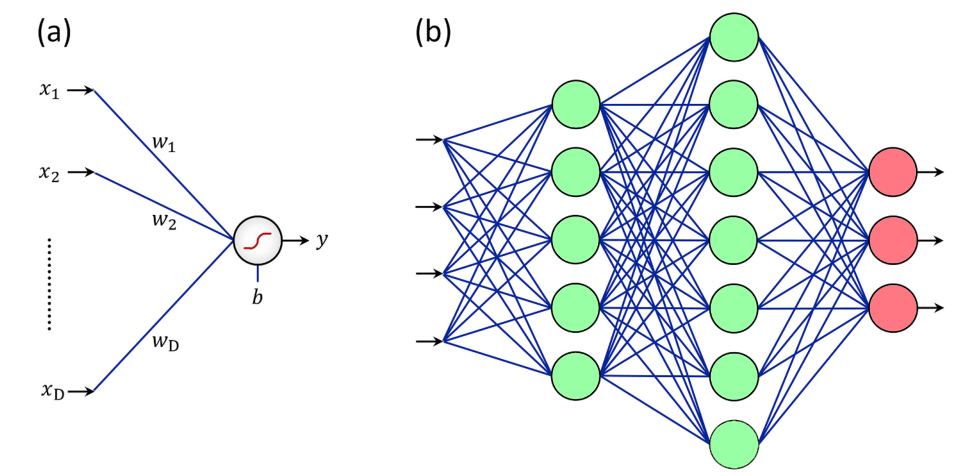
\includegraphics[scale=0.5]{figures/perceptron.png}
                
                \caption[The perceptron and multi-layer perceptron]{Illustration of a single neuron and a deep learning network of neurons.}
              	\medskip 
                \hspace*{15pt}\hbox{\scriptsize Credit: \citeauthor{razavi2021deep_exp_DL}\cite{razavi2021deep_exp_DL}}
                \label{Perceptron / MLP}
            \end{figure}
        
        The \textit{architecture} of any \gls{ann} consist of an input layer, a user-defined number of \textit{hidden layers} and finally an output layer\cite{razavi2021deep_exp_per}. More hidden layers, create a \textit{deeper} network, hence the name \textbf{deep learning}. An \gls{mlp} is a type of network called a \textit{feed-forward} \gls{ann} because the data flows from the input to the output layer and each layer is a function of the previous layer. During training, the weights between every neuron and the bias are optimized in a process which is further explained in section \ref{training neural networks}. The idea behind an MLP depicted in \ref{Perceptron / MLP} is that different neurons will activate with varying strengths depending on the input, resulting in different outputs. The architecture of the \gls{mlp} in figure \ref{Perceptron / MLP} can be expressed as\cite{Goodfellow-et-al-2016_architecture}:
        
        \begin{equation}
            \textbf{h}^{(1)} = \sigma^{(1)}(\textbf{W}^{(1)T}\textbf{x} + \textbf{b}^{(1)})
        \end{equation}
        \begin{equation}
            \textbf{h}^{(2)} = \sigma^{(2)}(\textbf{W}^{(2)T}\textbf{h}^{(1)} + \textbf{b}^{(2)})
        \end{equation}
        \begin{equation} \label{mlp outputlayer eq}
            \hat{\textbf{y}} = \sigma^{(3)}(\textbf{W}^{(3)T}\textbf{h}^{(2)} + \textbf{b}^{(3)})
        \end{equation}
        
        where for each layer \textbf{h} is a vector of activations, \textbf{W} is a vector of weights, \textbf{b} is a  vector of \textbf{biases}, and $\hat{\textbf{y}}$ is a vector of outputs. The activation function $\sigma$ can also vary from layer to layer.
        
        
    \subsection{Activation Function} \label{activation function}
        The activation function enables \gls{ann}s to learn non-linear features \cite{razavi2021deep_exp_per}. The reason it is needed is that a network consisting of only linear layers will be the same as a single linear layer \cite{razavi2021deep_exp_per}, and won't be able to capture non-linearities in the data, and therefore an activation function is required. The activation function used in this thesis was ReLU, which stands for \textit{rectified linear unit}, as described in \citeauthor{sharma2019new_activation_func}\cite{sharma2019new_activation_func}. ReLU simply takes a real number as input, and outputs this number if it is above zero, and otherwise it will output zero. Letting sigma denote the activation function, and x the input, the ReLU activation function can be formulated as follows:
            \begin{equation} \label{relu_eq}
                \sigma(x) = max(0,x)
            \end{equation}
        ReLU is also visualized in figure \ref{activation_fig}. Thus, this activation function allows some neurons to propagate their input, while preventing others from doing so. This can result in greater efficiency and faster training, as not all neurons are active, further detailed in \citeauthor{sharma2019new_activation_func}\cite{sharma2019new_activation_func}. 
        
        The sigmoid activation function transforms all input values to values in the range [0…1].\cite{sharma2019new_activation_func}. It could be applied to the output to solve binary classification problems, as the values can be treated as probabilities. The formula for sigmoid is:
            \begin{equation} \label{sigmoid_eq}
                \sigma(x) = \dfrac{1}{e^{-x}} 
            \end{equation}
            
            \begin{figure}[H]
                \centering
                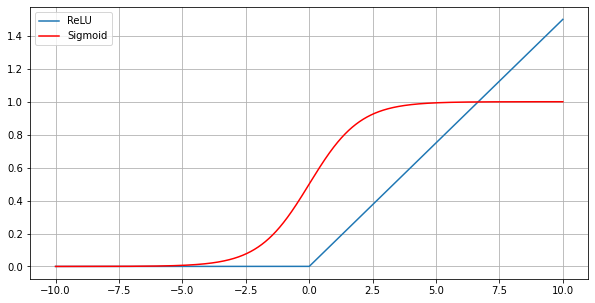
\includegraphics[scale=0.5]{figures/activation.png}
                \caption[ReLu and sigmoid]{A ReLU function (blue) and a sigmoid function (red)}.
              	\medskip 
                \label{activation_fig}
            \end{figure}
            
            
    \subsection{The Softmax Function}
        The \textit{softmax} function is a collection of many sigmoid functions, which allows it to solve problems containing multiple classes\cite{sharma2019new_activation_func}. For all data points, it calculates the probability of every class and can be expressed as:
        \begin{equation}
            \sigma(\textbf{x})_{j} = \dfrac{e^{x_{j}}}{\sum^{K}_{k=1}e^{x_{k}}} \textrm{ for j = 1,...,K.}
        \end{equation}
        
        where K is the number of classes and the output summarizes to 1 over all classes. For a network solving multiclass classification, the output layer will have size equal to K, which in figure \ref{Perceptron / MLP} corresponds to 3 classes. The \textit{softmax} would then be used as the last transformation ($\sigma^{(3)}$ in equation \ref{mlp outputlayer eq}) and output the probability of an input belonging to one of the three classes.

\section{Training Neural Networks} \label{training neural networks}
    This section will describe the main concepts behind how a machine learning algorithm using \gls{ann}s increase their performance on a task. 

\subsection{Forward-Propagation And The Loss Function}
    \citeauthor{Goodfellow-et-al-2016_NN}\cite{Goodfellow-et-al-2016_NN} describes \gls{ann} as an unknown function \textit{\^{f}} that maps an input \textbf{x} to an output \textbf{y}. The goal is to approximate some optimal function \textit{f} through learning from examples. In supervised tasks, the labels instruct the output layer exactly how to perform given the input data. However, the data does not inform the individual \textit{hidden layers} how to perform to produce this desired output. When the data flow through the network using the initial parameters $\theta$ (weights and biases), it produces outputs \textbf{\^{y}}, this is called the \textit{forward-propagation step}. How the parameters are initialized can heavily affect the training process, and different strategies are further described in \citeauthor{Goodfellow-et-al-2016_param_init}\cite{Goodfellow-et-al-2016_param_init}. By using a \textit{loss function} comparing the true \textbf{y} values to the estimated values \textbf{\^{y}}, we get a measurement of the network's \textit{error}, also called \textit{loss}. In classification tasks, the network is trained to output the probability of each class given an input\cite{ho2019real_weighted_cross_entropy}. The probabilities are then the input to the loss function, which in this work is \textit{weighted cross entropy}. This function outputs a loss based on probabilities, weights classification of certain classes differently, and is often used when dealing with data containing class imbalance as you can apply more weight to the minority class. Expressed as:
    
        \begin{equation} \label{cross_entropy}
            loss(\theta) = - \sum^{n}_{i=1} w_{y_{i}}y_{i}\log(\hat{y_{i}})
        \end{equation}
    
    where \textit{n} is the number of classes, $y_{i}$ is the true value, $\hat{y_{i}}$ is the output from the softmax for the $i^{th}$ class, and $w_{y_{i}}$ is the weight of the class to which $y_{i}$ belongs. More examples of loss functions can be viewed in \citeauthor{mishra2017deep}\cite{mishra2017deep}.
    


\subsection{Stochastic Gradient Decent} \label{batch learning}
        \begin{quote}
        "\textit{A recurring problem in machine learning is that large training sets are necessary for good generalization, but large training sets are also more computationally
        expensive."} - (\citeauthor{Goodfellow-et-al-2016_SGD}\citeyear{Goodfellow-et-al-2016_SGD}, page 152)
    \end{quote}
    
    The problem, described in the quote above, arises when we have a large dataset, and we would calculate the loss values of all samples before updating the parameters in our network\cite{Goodfellow-et-al-2016_SGD}. Depending on the hardware, this could lead to a crash or slow learning due to heavy memory demands. A solution is then to sample examples from the entire dataset with a uniform distribution, hence forming a \textit{mini-batch}, with the intent to approximately estimate the true \textit{loss} using this smaller fraction of the dataset. Then we update the parameters of our network based on this and repeat on a new batch. When we have run this process on all the data, we say that an \textit{epoch} has passed. The size of this minibatch can vary from one example, to hundreds, and the size chosen can heavily affect training\cite{wilson2001need_learning_rate}. A widely used algorithm is \textit{\gls{sgd}}\cite{Goodfellow-et-al-2016_SGD}, which utilizes this minibatch form of training, and is used in this thesis. In the more precise form, \gls{sgd} batch learning is formulated as\cite{pmlr-v37-ioffe15_batch_norm}:
    
        \begin{equation} \label{batch_learning_eq}
            \theta = \arg \min_{\theta}\dfrac{1}{N} \sum^{N}_{i=1} loss (x_{i},\theta)
        \end{equation}
    
    where $\theta$ is the set of parameters to be optimized, $x_{1..N}$ is the training data, and $x_{1..m}$ is a minibatch of the training data. \gls{sgd} is what is called an \textit{optimization} algorithm, and the next section will describe how it is applied to solve equation \ref{batch_learning_eq}. 
    
    
\subsection{Backpropagation And Gradient-based Learning}
    To update the parameters of the network, we use the loss from a batch, and iteratively step back through the layers in a process called \textit{back-propagation}\cite{rumelhart1986learning_backprop}. In each step, we calculate a value called the \textit{gradient} for each parameter. The gradient is the partial derivative of the \textit{loss} function with respect to each weight and bias in the current layer, and is computed using the chain rule. This is in order to determine how changes to each parameter will affect the \textit{loss}. Using the gradient, \gls{sgd} adjusts all the individual parameters to minimize the \textit{loss}, performing \textit{gradient descent}\cite{Goodfellow-et-al-2016_gradient_descent} by updating all parameters in the opposite direction of the gradient to reduce the \textit{loss}. In what magnitude a parameter is adjusted by the optimizing algorithm is determined by the \textit{learning rate}, usually a value between 0 and 1. The parameter update is expressed as\cite{pmlr-v37-ioffe15_batch_norm}:
    
    \begin{equation}
    \theta^{(j)} \leftarrow \theta^{(j)} - \varepsilon \dfrac{1}{m}\sum_{i=1}^{m} \dfrac{\partial loss (\theta^{(j)})}{\partial \theta^{(j)}}
    \end{equation}
    
    where $\theta$ is the parameters of the nework, \textit{m} is the batch size, $\varepsilon$ is the learning rate, and \textit{j} is the layer. In figure \ref{learning_rates} an example loss function is illustrated with one global \textit{loss} minima, and different learning rates applied with \gls{sgd}. Low learning rate values usually have a long training time, and can even cause the \gls{sgd} to find some local minima instead of the global\cite{farsal2018deep}. However, too high values can overshoot the global minima and diverge. Both can be prevented by applying a method to adapt the learning rate to the \textit{topography} of the loss function. In this thesis, \textit{momentum} was applied, which adds a \textit{velocity} parameter to the update step. This \textit{velocity} is based on past steps and the update will step in the \textit{velocities'} direction, not the current \textit{gradient}. More detail on \textit{momentum} can be found in \citeauthor{pmlr-v28-sutskever13}\cite{pmlr-v28-sutskever13}.
    
    \begin{figure}[H]
        \centering

        \includesvg[inkscapelatex=false,width=1.0\textwidth,keepaspectratio]{figures/learning_rates.svg}
        \caption[Learning rates]{Three different applications of \gls{sgd} on a loss function . Each arrow is an imagined learning step taken by the algorithm for; (a) low learning rate, (b) high learning rate, and (c) momentum.}
      	\medskip 
        \label{learning_rates}
    \end{figure}

    In summary, the entire training process using \gls{sgd} can be described as the following algorithm\cite{farsal2018deep}:
    
    \begin{longtable}{lllllll} \label{sgd algorithm}\\
    \hline
    \multicolumn{7}{l}{Mini-batch SGD one epoch}                                                              \\ \hline
    \endfirsthead
    %
    \endhead
    %
    \hline
    \endfoot
    %
    \endlastfoot
    %
    \multicolumn{7}{l}{Loop:}                                                                       \\
    1.   & \multicolumn{6}{l}{Sample batch of data.}                                                \\
    2.   & \multicolumn{6}{l}{Forward propagate the batch through the network and compute the loss.} \\
    3.   & \multicolumn{6}{l}{Back propagate to calculate the gradients.}                            \\
    4.   & \multicolumn{6}{l}{Update the parameters based on the gradients.}                         \\ \hline
    \end{longtable}
    
    

%\subsection{Vanishing and exploding gradient} \label{}
    %By repeatedly applying forward-propagation, back-propagation and some optimizing algorithm on new examples as stated by \citeauthor{Goodfellow-et-al-2016_NN}, you train a network to approximate the optimal function \textit{f}.
    
\subsection{Regularization}
    Regularization as described by \citeauthor{kukavcka2017_regularization}\cite{kukavcka2017_regularization} is a small alternation or technique added to the training process that has as goal to make the model generalize better. This can be applied in different ways, and two used in this thesis will be described here; \textit{batch normalization} and \textit{data-augmentation}.
    
\subsubsection{Batch-Norm}
    Batch normalization is a technique applied to reduce what is called \textit{internal  covariate shift}\cite{pmlr-v37-ioffe15_batch_norm}. This is defined as the change in the distribution of activations in \gls{ann}s hidden layers caused by the change in the networks parameters when training. During \textit{backpropagation}, the hidden layers depend on the activations of all layers before them, and this has been shown to slow down and destabilize the training process. The solution to this problem is the implementation of \textit{batch normalization}. By using the activations from all the neurons in a hidden layer, a \textit{mean} and \textit{variance} is calculated per batch. These values are then used to normalize the activations of the hidden layer, and each hidden layer are given two additional learnable parameters $\gamma$ and $\beta$, that perform a linear transformation of the normalized activations, defined as such:
    
        \begin{equation} \label{batch_normalization}
            \hat{Z}^{(i)} =   \gamma Z^{(i)}_{norm} + \beta
        \end{equation}
    
    where $\hat{Z}^{(i)}$ is the batch normalized activations, $Z^{(i)}_{norm}$ is the normalized activations for the $i^{th}$ hidden layer. The learnable parameters make the \gls{ann} able to adjust and shift the distribution through the training process. The result is a faster and more stable training process. 

\subsubsection{Data-Augmentation} \label{data-augmentation}
    The previous regularization method is applied during training, but \textit{data-augmentation} is applied to the training dataset\cite{kukavcka2017_regularization}. There are several methods available, but the two used in this work are: \textit{adding noise} and \textit{vertical flipping}. One example of applying noise is to add Gaussian values with a mean of 0 and some user-defined variance to each pixel. This adds more randomness to the data, making the model learn more general features instead of specific, hence increasing generalization performance. Other methods of applying noise are described in \citeauthor{kukavcka2017_regularization}\cite{kukavcka2017_regularization}. The \textit{flipping} is a simple yet effective transformation where we flip the input and label along a certain axis, and now produce a new sample. During training, an echograms' orientation of the surface and bottom can never individually be changed, and so vertical flipping is justified in on acoustic data. This is an important observation when applying data augmentation, as it can't change the meaning of the data. For example, when classifying numbers in images, rotating an image of the number \textit{9} clockwise 180 degrees will change its representation to now be more similar to a \textit{6}, but the label would still say it belongs to the class \textit{9}. An example of each method mentioned can be seen in figure \ref{data augmentation fig}:
    
    \begin{figure}[H]
        \centering
        
        \subfloat[Gaussian noise added to each pixel.]{
        	\includesvg[inkscapelatex=false,width=0.9\textwidth,keepaspectratio]{figures/add_noise.svg}}
        	%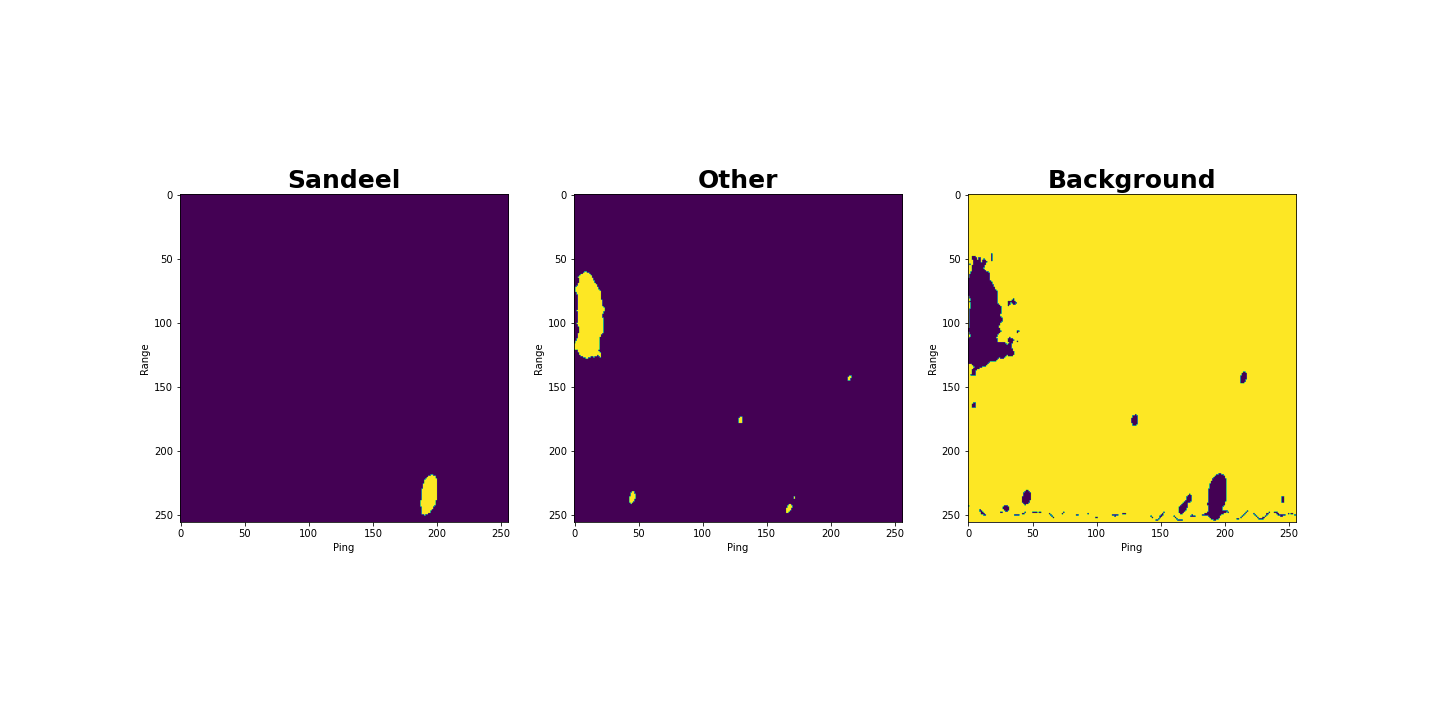
\includegraphics[width=1\textwidth]{figures/data_sample.png} } 
        
        \subfloat[Vertical flipping.]{
        	\includesvg[inkscapelatex=false,width=0.9\textwidth,keepaspectratio]{figures/vertical_flip.svg}}
        
        
        \caption[Two data augmentation examples]{Two augmentation methods applied to the same image.}
        \label{data augmentation fig}
        
        \end{figure}
    
    
\clearpage
\section{Computer Vision} \label{computer vision}
    \textbf{Computer vision} is a very popular field of research within deep learning\cite{voulodimos2018deep_computer_vision}. This is because it has mainly focused on tasks we humans do seemingly without training, while computers struggle with it. Examples are facial recognition, object detection. There are also works that have gone beyond human capability, like \citeauthor{davis2014visual_deep_video_audio}s\cite{davis2014visual_deep_video_audio} work, where they recovered sounds from the vibrations they induced in objects captured on video. There are many methods in the field of computer vision, but we will focus on the \gls{cnn}. 
    
    
    
\subsection{Convolutional Neural Network} \label{cnn}
    \gls{cnn}s are a type of \gls{ann}s that are primarily used in machine learning tasks concerning images\cite{o2015introduction_convolutions}.The need for the convolutional operation stemmed from the fact that images input to a regular \gls{ann} produces a large amount of learnable parameters. A low-resolution image with 512×512 pixels passed to an input layer containing only one neuron would have $1*512*512 = 262144$ weights alone.  To solve this issue and have fewer learnable parameters, the \gls{cnn} is built around 3 main components\cite{o2015introduction_convolutions}; \textit{convolutional layer}, \textit{pooling layer} and a \textit{fully-connected layer}. An example \gls{cnn} is illustrated in figure \ref{convolutional_neural_network_fig} and each main component will be explained later in this section.

    \begin{figure}[H]
        \centering
                        \includesvg[inkscapelatex=false,width=0.95\textwidth,keepaspectratio]{figures/conv_net.svg}
        \caption[Convolutional neural network example]{Illustrations of the main components in a \gls{cnn}. The \textit{flatten} operation is applied here to make the output from the pooling layer compatible with the fully connected layer of regular neurons.}
      	\medskip 
        \label{convolutional_neural_network_fig}
    \end{figure}
    
    \subsubsection{Convolutional Layer}
     \citeauthor{o2015introduction_convolutions}\cite{o2015introduction_convolutions} describe the convolutional layer as consisting of a number of learnable multidimensional weight matrices. Henceforth, we will refer to such a matrix as a kernel. The height and the width of the kernel are parameters defined by the user, but the depth will always equal the number of channels in the input. This results in kernels being described only by \textit{height} x \textit{width}. The kernel slides over the input, and is applied to different locations of the input, also called the current \textit{receptive field}. When applied, a single scalar value is computed that is the weighted sum of the kernel's weights and the corresponding values in the receptive field. If we have a 2-dimensional image $S(i,j)$ as input, a convolutional operation would be expressed as\cite{Goodfellow-et-al-2016_convolution}:
     
        \begin{equation}
            S(i,j) = (I*K)(i,j) = \sum_{height}\sum_{width}I(i+height,j+width)K(height,width)
        \end{equation}
     
     where $*$ is the convolutional operation, I is the input and K is the kernel.
     
     The output scalar value from the convolutional operation is called the \textit{activation}, and is often fed through non-linear activation functions like ReLU\cite{o2015introduction_convolutions}. The sliding operation is constructed around a value called \textit{stride}, which is the number of horizontal positions to move the kernel in the input between each calculation. If it is not possible to move in the horizontal direction, the kernel will move rows down vertically equal to the stride and begin anew. After sliding over the entire input, a complete 2-dimensional activation map has been created, one such map for each kernel applied and often several is applied. The idea is that each of these kernels will learn to identify different features in the input, and an example of a horizontal edge detector can be seen in figure \ref{convolutional_fig}. 
    \begin{figure}[H]
        \centering
                \includesvg[inkscapelatex=false,width=0.9\textwidth,keepaspectratio]{figures/convolutions.svg}
        \caption[Horizontal edge detector example]{Illustration of a \textit{valid} convolutional operation. The kernel is applied repeatedly across the input. The size of input is 6x6, kernel size is 3x3 and stride 1, resulting in overlapping operations and output size being 4x4. The figures to the right show the input, kernel and output(activation) as color gradings, where the color gets darker if the values are low. This example is a horizontal edge detector, and the result is large values in the activation map along the border between the values of 0 and 10 in the input, which could have been colors in a picture.}
      	\medskip 
        \label{convolutional_fig}
    \end{figure}
    
    The receptive field will start as small regions, but as we apply more convolutional layers, it will have access to increasing context in regard to the input\cite{o2015introduction_convolutions}. This is illustrated in figure \ref{receptive_field_fig}, and kernels in early layers learn to identify simple features while later combine these to identify complex features. In the same figure, this could for example have been the upper and lower jaw of the leftmost cat being combined to recognize a mouth in later layers. The kernel is slid over its entire input and so utilizes what is called \textit{parameter sharing }, as the same weights are used repeatedly across the input. Another positive consequence is that the location of the feature in the input is not relevant to a convolutional neural network. Combined, this creates a layer able to detect features in an input with fewer learnable parameters than a normal \gls{ann}. 
    
    \begin{figure}[H]
        \centering
        \includesvg[inkscapelatex=false,width=0.9\textwidth,keepaspectratio]{figures/receptive_field.svg}
        
        \caption[Receptive field]{The activation maps from two convolutional layers with 3×3 kernels and stride 1. The first convolution's receptive field is marked as red. On its activation map, a new convolutional layer is applied. Its first receptive field is outlined in green, which translates to a larger area in the input.}
      	\medskip 
        \label{receptive_field_fig}
    \end{figure}

    %The complete \textit{convolutional operation} performed by a convolutional layer consists of applying this kernel to the entire input. Producing activations for different regions of the input. This reduces the dimension of the input to a 2D activation output, but you may apply several kernels to increase the channels, as each will create a new 2D channel in the activations. A convolutional operation is often followed up with an element wise nonlinear activation function to its activations, like a ReLu. The kernels will through training learn to detect different features in the input, and so in a \gls{cnn} the first layers will often detect simple features like edges. Later layers will then detect more complex features like cars and houses, combining the activations from different earlier layers. The last layer consists of a \textit{fully connected} layer of regular neurons to determine the output, but implementations of networks with only convolutional operations exists like U-Net which will be described\cite{unet_ronneberger2015} in section \ref{unet} utilizing 1x1 convolutions. A more detailed example can be found in figure \ref{convolutional_fig} which looks at how a convolution with a horizontal edge detecting kernel is applied to a single channel or an equivalent 2D input. 
    
    Reductions in the spatial size\cite{o2015introduction_convolutions} will normally occur with the convolutional operation described so far in this section, and this type is called \textit{valid convolutions}. By applying a padding with zeros around the input, we can retain the dimensions of the input. The effect is that more convolutional operations fit in the new padded input, hence a larger output size. This is called a \textit{same convolution}. Illustrated in figure \ref{same_convolutional_fig}.
    
    \begin{figure}[H]
        \centering
        \includesvg[inkscapelatex=false,width=0.9\textwidth,keepaspectratio]{figures/same_convolutions.svg}
        \caption[Same convolution example]{Illustration of a \textit{same} convolutional operation. The size of the input is 3×3, but after padding with zeros the size is 5×5, kernel size is 3×3 and stride is 1. Resulting in an activation map if size 3×3, hence conserving the input size.}
      	\medskip 
        \label{same_convolutional_fig}
    \end{figure}
    
    
    
\subsubsection{Pooling Layer}

    \begin{figure}[H]
        \centering
                \includesvg[inkscapelatex=false,width=0.8\textwidth,keepaspectratio]{figures/maxpool.svg}
        \caption[The max pool operation]{Illustration of the max pool operation with size 2×2 and stride 2.}
      	\medskip 
        \label{maxpool_fig}
    \end{figure}
    There are different pooling layers, but we will focus on the variant called \textit{max pool} used in this thesis. The max pool layer reduces the \textit{height} and \textit{widht} of its input\cite{o2015introduction_convolutions}. Like a convolutional operation, the max pool looks at a region of the input, but instead applies a \textit{max} operation. The pooling kernel size is given in \textit{height} x \textit{width}, and is applied individually to each dimension of the input. This reduces the height and width, but not the channels. The most common setting is 2×2 with a stride 2, which results in decreasing the resolution to 25\% of the original size. Alone, the max pool has no learnable parameters and is applied with the purpose of decreasing the computation complexity of the \gls{cnn}.


\subsubsection{Fully Connected Layer}
    \begin{figure}[H]
        \centering
        \includesvg[inkscapelatex=false,width=0.95\textwidth,keepaspectratio]{figures/1x1.svg}
        %\includesvg[inkscapelatex=false,scale=0.3,keepaspectratio]{figures/Bilde1.svg}
        \caption[1×1 convolution]{Illustration of the 1×1 convolution with stride 1.}
      	\medskip 
        \label{1x1_fig}
    \end{figure}
    \citeauthor{lin2013network_in_network_1x1}\cite{lin2013network_in_network_1x1} proposed the convolutional layer with kernel size 1×1 and stride 1, followed by an activation function, as an equivalent to the regular hidden layer shown earlier in figure \ref{Perceptron / MLP}. The 1×1 layer will take the weighted sum along a 1×1 slice through all channels of the input, as illustrated in figure \ref{1x1_fig}. This is equivalent to applying a fully connected layer to the same values. As this preserves the \textit{resolution}, it can be used as a tool for alterations of the depth of the output feature maps by specifying the desired number of kernels. In figure \ref{1x1_fig} we have only one kernel, but if two were applied instead, the output feature map would have a depth of two. In this work, it is used mainly to map high dimensional feature maps to the desired number of classes.
    
    

\subsubsection{Transposed Convolutions}
    \begin{figure}[H]
        \centering
        \includesvg[inkscapelatex=false,width=0.95\textwidth,keepaspectratio]{figures/transpose_conv.svg}
        
        
        \caption[Transposed convolution]{Illustration of the transposed convolution operation with kernel size 2×2 and stride 1. The green color shows one of the intermediate computations. The center value of each crop is outlined to illustrate the summation step as these overlap.}
      	\medskip 
        \label{transposed_conv_fig}
    \end{figure}
    A transposed convolution is an operation performing the opposite operation compared to a regular convolution\cite{dumoulin2016guide_transposed_convolution}. This means taking an input, and with a kernel similar to that described in \ref{cnn} now instead map the input to a higher resolution. In example figure \ref{transposed_conv_fig}, a 2-dimensional 2×2 input is fed to a transposed convolutional layer with kernel size 2×2. The whole kernel is multiplied element-wise to the input and proceeds to produce values in a temporary matrix initialized with zeros, denoted by empty cells in the figure. The calculated values in the temporary matrix are situated correctly relative to the input. These temporary matrices are then summed over, producing the output. This operation is repeated for all channels, retaining the depth of the input. 
    

    
\subsubsection{Segmentation}
    \begin{figure}[H]
        \centering
        \includesvg[inkscapelatex=false,width=0.95\textwidth,keepaspectratio]{figures/segmentation.svg}
        \caption[Difference between semantic and instance segmentation]{Illustration of the difference between semantic and instance segmentation.}
      	\medskip 
        \label{segmentation_fig}
    \end{figure}

    Segmentation is a computer vision task where the objective is to assign one or several classification masks to the input\cite{He_2017_ICCV_segmentation}. This is again split into two different categories: \textit{semantic} and \textit{instance} segmentation. In semantic segmentation, we assign each pixel in the input to predefined classes. Regarding the example figure \ref{segmentation_fig}, this could be done by utilizing a \gls{cnn}. The output would have the same resolution as  the input, but with depth equal to the number of classes. A softmax would then be calculated for each pixel across the depth, and the pixel would be assigned to the class with the highest probability. Hence, producing a mask of each class. In instance segmentation, we increase the complexity by applying semantic segmentation and in parallel assigning a bounding box to each individual object, as visualized in the example figure. Semantic segmentation is the method applied in this thesis, thus no further details concerning instance segmentation is necessary.
    

    


        

    
    